
%(BEGIN_QUESTION)
% Copyright 2006, Tony R. Kuphaldt, released under the Creative Commons Attribution License (v 1.0)
% This means you may do almost anything with this work of mine, so long as you give me proper credit

Tegn væskestrømmen ($Q$) inn i denne tanken, gitt grafen for akkumulert væskevolum ($V$) over tid. Funksjonen du tegner (som beskriver væskestrøm) vil være den {\it tidsderiverte} av funksjonen som vises (som beskriver væskevolum):

$$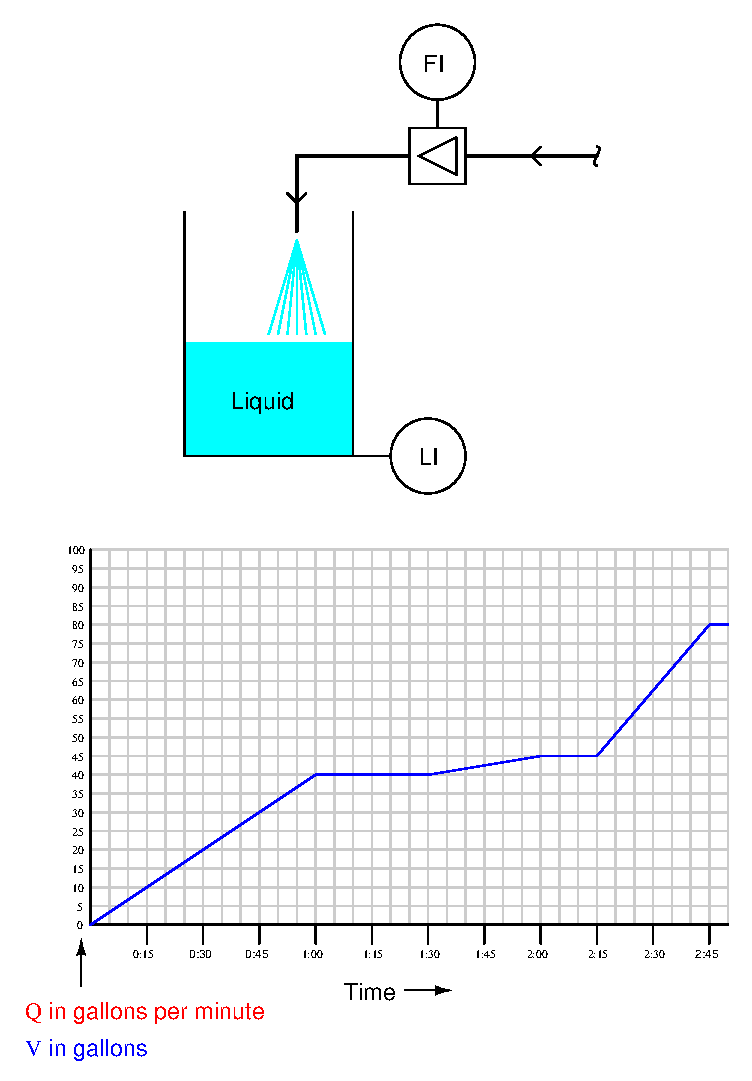
\includegraphics[width=15.5cm]{i01531x01.eps}$$

\underbar{file i01531}
%(END_QUESTION)





%(BEGIN_ANSWER)

$$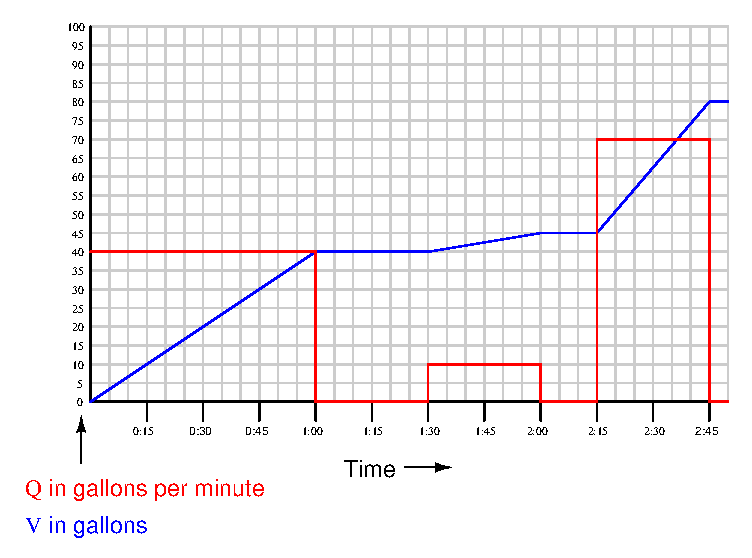
\includegraphics[width=15.5cm]{i01531x02.eps}$$

Perioder der volumet øker lineært (rettlinjet stigning) indikerer en konstant væskestrøm inn i tanken. For å beregne denne strømningsraten måler du endring i volum ($\Delta V$) og deler på endring i tid ($\Delta t$), altså stigning over løp.

\vskip 10pt

Mellom 0:00 og 1:00 økte volumet jevnt fra 0 gallon til 40 gallon i løpet av 1 minutt. Derfor var strømningsraten i denne perioden 40 gallon per minutt.

\vskip 10pt

Mellom 1:00 og 1:30 var volumet konstant. Dette indikerer en periode uten væskestrøm inn i tanken, så strømningsraten her er 0 gallon per minutt.

\vskip 10pt

Mellom 1:30 og 2:00 økte volumet jevnt fra 40 gallon til 45 gallon i løpet av 0.5 minutter (1/2 minutt). Derfor var strømningsraten i denne perioden 10 gallon per minutt.

\vskip 10pt

Mellom 2:00 og 2:15 var volumet konstant. Igjen indikerer dette en periode uten væskestrøm inn i tanken, så strømningsraten her er 0 gallon per minutt.

\vskip 10pt

Mellom 2:15 og 2:45 økte volumet jevnt fra 45 gallon til 80 gallon i løpet av 0.5 minutter (1/2 minutt). Derfor var strømningsraten i denne perioden 70 gallon per minutt.

\vskip 10pt

Mellom 2:45 og slutten av grafen var volumet konstant. Ingen strøm inn i tanken her (0 gallon per minutt).

%(END_ANSWER)





%(BEGIN_NOTES)


%INDEX% Mathematics, calculus: derivative (calculating flow rates from measured volumes at specific times)

%(END_NOTES)

